% 图 46.1 —— 由 `checks/emit_hand.py` 自动拼出（probe 精测 + prims2 图元分解）
%%
% ⚠ 这是**稿子不是成品**：跑 `checks/checkhand.py 46.1` 看指标 + 看叠合图。
%%
%% ⚠ 待核：
%   · 本图 probe 报出阴影族 1 个 —— **本脚本不生成阴影**（要照原书手写）；prims2 的 strokes 里可能含阴影线，核对时留意别画重
%   · 可疑字形 1 项（空心圈 ⊙ 常被认成字母 o）—— 见文件末
%%
\documentclass[12pt]{standalone}
\usepackage{fontspec}
\setsansfont{Arial}
\newfontfamily\mfallback{DejaVu Sans}
\usepackage{tikz}
\begin{document}
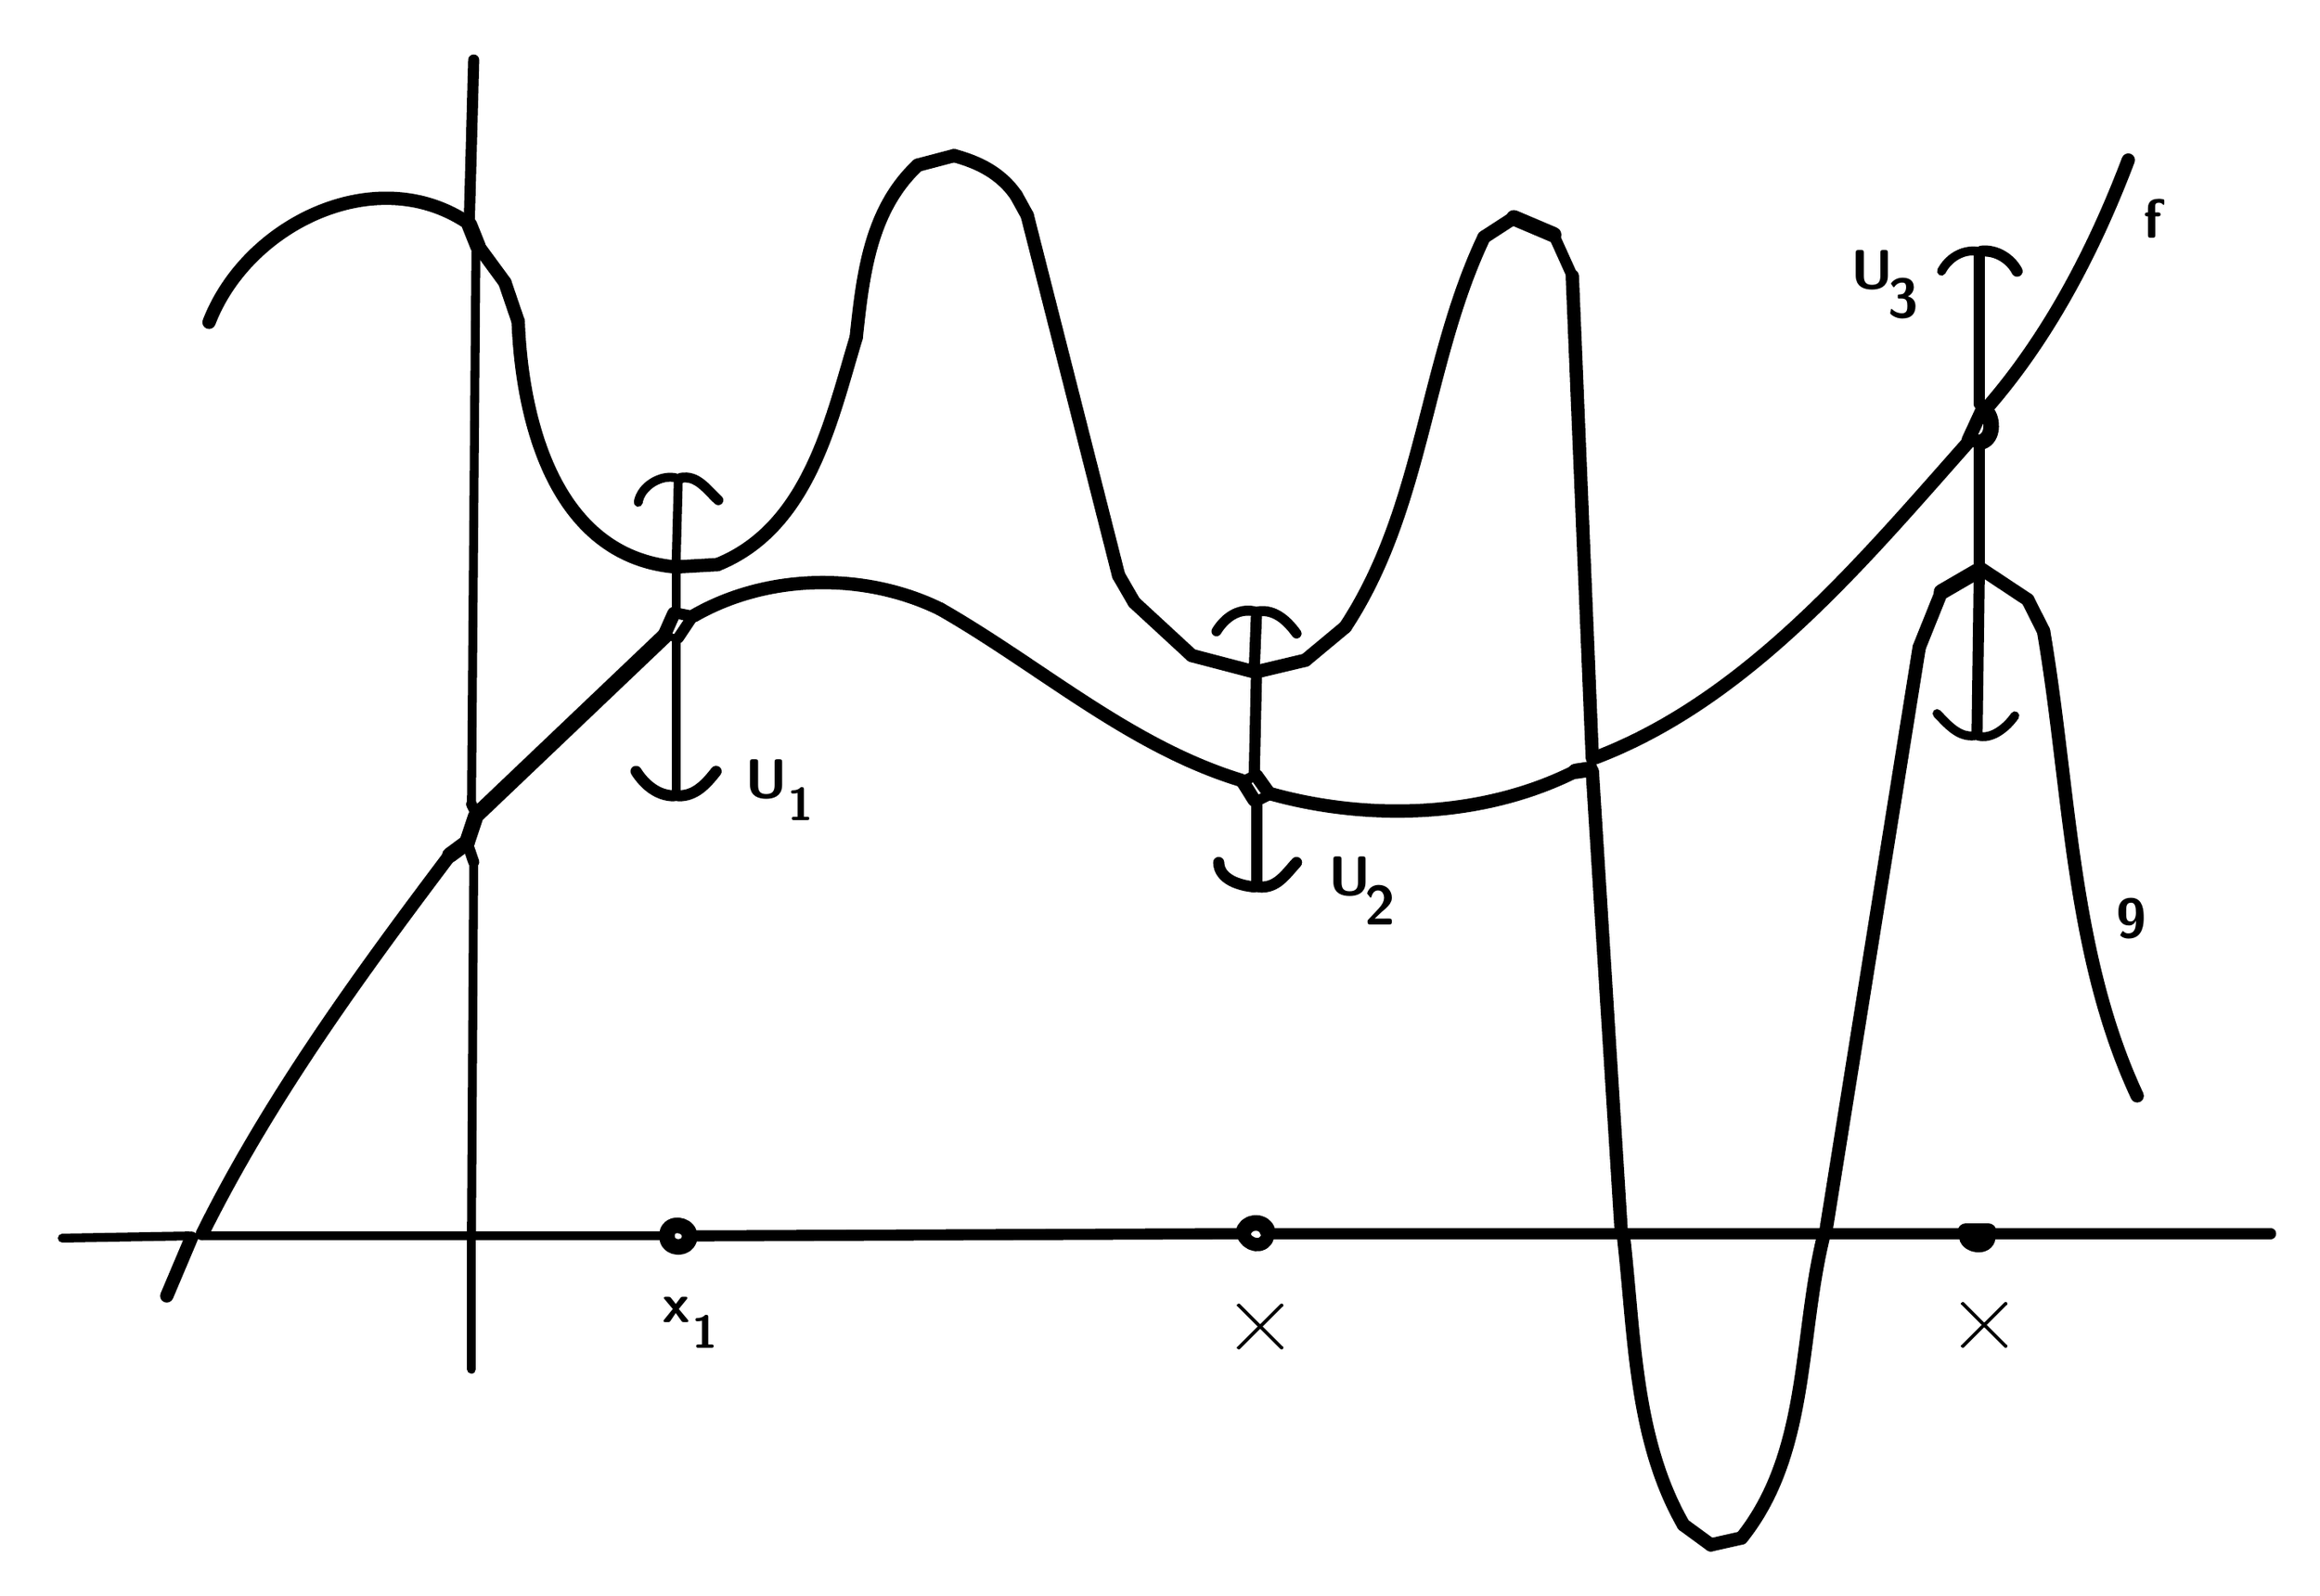
\begin{tikzpicture}[x=1pt, y=-1pt, line width=4.0pt, line cap=round, line join=round]

  %% ════ 直线段（prims2 的 strokes）════
  \draw[line width=4.0pt] (75.0,546.0) -- (18.0,547.0);
  \draw[line width=4.0pt] (203.0,546.0) -- (289.0,546.0);
  \draw[line width=4.7pt] (554.0,339.0) -- (550.0,341.0);
  \draw[line width=4.0pt] (202.0,547.0) -- (202.0,606.0);
  \draw[line width=6.0pt] (65.0,573.0) -- (76.0,547.0);
  \draw[line width=5.0pt] (880.0,104.0) -- (880.0,171.8);
  \draw[line width=3.0pt] (880.0,171.8) -- (882.0,174.0);
  \draw[line width=6.0pt] (289.0,275.0) -- (293.0,266.0);
  \draw[line width=5.0pt] (549.0,545.0) -- (301.0,546.0);
  \draw[line width=6.9pt] (698.4,337.0) -- (705.0,336.0);
  \draw[line width=5.0pt] (879.0,320.0) -- (880.0,248.0);
  \draw[line width=6.0pt] (223.0,134.6) -- (217.0,117.0);
  \draw[line width=6.0pt] (217.0,117.0) -- (206.0,102.0);
  \draw[line width=4.0pt] (294.0,244.0) -- (295.0,206.0);
  \draw[line width=7.0pt] (201.0,91.0) -- (205.0,101.0);
  \draw[line width=6.0pt] (881.0,175.0) -- (875.0,188.0);
  \draw[line width=6.0pt] (908.9,273.9) -- (901.8,259.8);
  \draw[line width=6.0pt] (901.8,259.8) -- (881.0,246.0);
  \draw[line width=4.0pt] (294.0,246.0) -- (294.0,265.0);
  \draw[line width=3.0pt] (879.0,189.0) -- (876.0,189.0);
  \draw[line width=5.0pt] (718.0,545.0) -- (561.0,545.0);
  \draw[line width=6.0pt] (556.0,292.0) -- (577.0,287.0);
  \draw[line width=6.0pt] (577.0,287.0) -- (594.9,272.1);
  \draw[line width=6.0pt] (657.3,96.7) -- (670.7,88.0);
  \draw[line width=7.0pt] (670.7,88.0) -- (688.6,95.6);
  \draw[line width=5.0pt] (688.6,95.6) -- (697.0,114.2);
  \draw[line width=6.0pt] (697.0,114.2) -- (706.0,331.0);
  \draw[line width=6.0pt] (719.0,544.0) -- (706.0,337.0);
  \draw[line width=4.0pt] (294.0,278.0) -- (294.0,347.0);
  \draw[line width=4.8pt] (204.0,356.0) -- (202.0,351.8);
  \draw[line width=4.0pt] (202.0,351.8) -- (204.0,103.0);
  \draw[line width=7.5pt] (874.0,544.0) -- (884.0,544.0);
  \draw[line width=5.0pt] (295.0,266.0) -- (300.0,267.0);
  \draw[line width=6.0pt] (554.0,350.0) -- (549.0,342.0);
  \draw[line width=5.0pt] (295.0,277.0) -- (301.0,268.0);
  \draw[line width=3.4pt] (290.0,276.0) -- (293.0,277.0);
  \draw[line width=3.0pt] (77.0,546.0) -- (80.0,546.0);
  \draw[line width=3.0pt] (706.0,332.0) -- (706.0,335.0);
  \draw[line width=5.0pt] (203.0,17.0) -- (201.0,90.0);
  \draw[line width=4.7pt] (556.0,350.0) -- (560.0,348.0);
  \draw[line width=6.0pt] (555.0,339.0) -- (560.0,346.0);
  \draw[line width=6.0pt] (295.0,245.0) -- (312.6,244.0);
  \draw[line width=6.0pt] (402.7,64.3) -- (419.0,60.0);
  \draw[line width=6.0pt] (447.0,78.0) -- (451.9,86.9);
  \draw[line width=6.0pt] (451.9,86.9) -- (493.0,248.9);
  \draw[line width=6.0pt] (493.0,248.9) -- (500.0,261.0);
  \draw[line width=6.0pt] (500.0,261.0) -- (525.9,284.9);
  \draw[line width=6.0pt] (525.9,284.9) -- (553.0,292.0);
  \draw[line width=5.0pt] (880.0,190.0) -- (880.0,245.0);
  \draw[line width=5.0pt] (809.0,545.0) -- (721.0,545.0);
  \draw[line width=5.0pt] (555.0,266.0) -- (554.0,291.0);
  \draw[line width=5.0pt] (873.0,545.0) -- (812.0,545.0);
  \draw[line width=6.0pt] (773.1,681.9) -- (759.3,685.0);
  \draw[line width=6.0pt] (759.3,685.0) -- (747.0,676.0);
  \draw[line width=5.0pt] (555.0,351.0) -- (555.0,388.0);
  \draw[line width=7.0pt] (289.0,276.0) -- (205.0,356.0);
  \draw[line width=5.0pt] (554.0,338.0) -- (555.0,293.0);
  \draw[line width=7.0pt] (204.0,357.0) -- (200.0,369.0);
  \draw[line width=7.0pt] (879.0,247.0) -- (863.0,256.3);
  \draw[line width=6.0pt] (863.0,256.3) -- (853.0,281.2);
  \draw[line width=6.0pt] (853.0,281.2) -- (811.0,544.0);
  \draw[line width=7.0pt] (200.0,369.0) -- (192.3,374.7);
  \draw[line width=5.0pt] (200.0,369.0) -- (203.0,377.8);
  \draw[line width=4.0pt] (203.0,377.8) -- (202.0,545.0);
  \draw[line width=5.0pt] (1011.0,545.0) -- (885.0,545.0);
  \draw[line width=4.0pt] (82.0,546.0) -- (201.0,546.0);

  %% ════ 曲线（prims2 的 curves —— 三段式，坐标同为 (y,x)）════
  \draw[line width=6.0pt] (875.0,189.0) .. controls (826.9,243.3) and (775.4,305.1) .. (707.0,331.0);
  \draw[line width=4.0pt] (878.0,321.0) .. controls (870.6,321.9) and (865.8,315.9) .. (861.0,311.0);
  \draw[line width=6.0pt] (560.0,546.0) .. controls (558.7,552.3) and (550.3,550.4) .. (549.0,545.0);
  \draw[line width=7.0pt] (549.0,545.0) .. controls (549.5,539.1) and (558.6,538.3) .. (560.0,544.0);
  \draw[line width=6.0pt] (947.0,62.0) .. controls (931.9,101.8) and (911.4,141.6) .. (883.0,174.0);
  \draw[line width=6.0pt] (561.0,347.0) .. controls (605.6,359.5) and (657.1,357.8) .. (698.4,337.0);
  \draw[line width=5.0pt] (573.0,378.0) .. controls (568.1,383.3) and (564.1,389.8) .. (556.0,389.0);
  \draw[line width=6.0pt] (293.0,245.0) .. controls (239.5,239.7) and (224.7,179.4) .. (223.0,134.6);
  \draw[line width=5.0pt] (312.0,337.0) .. controls (307.5,342.7) and (302.6,348.2) .. (295.0,348.0);
  \draw[line width=4.5pt] (313.0,215.0) .. controls (307.9,210.4) and (303.6,203.5) .. (296.0,205.0);
  \draw[line width=6.0pt] (951.0,483.0) .. controls (921.0,418.6) and (920.9,344.2) .. (908.9,273.9);
  \draw[line width=4.5pt] (554.0,265.0) .. controls (546.6,263.5) and (540.6,268.1) .. (537.0,274.0);
  \draw[line width=4.0pt] (879.0,103.0) .. controls (872.3,102.2) and (866.1,106.1) .. (863.0,112.0);
  \draw[line width=6.0pt] (594.9,272.1) .. controls (630.0,218.8) and (630.6,153.0) .. (657.3,96.7);
  \draw[line width=6.5pt] (884.0,546.0) .. controls (884.7,552.0) and (874.3,551.1) .. (874.0,546.0);
  \draw[line width=7.0pt] (883.0,175.0) .. controls (886.7,178.8) and (886.3,188.3) .. (880.0,189.0);
  \draw[line width=7.0pt] (300.0,547.0) .. controls (299.4,552.3) and (290.6,552.3) .. (290.0,547.0);
  \draw[line width=4.5pt] (556.0,265.0) .. controls (563.5,264.1) and (569.0,269.5) .. (573.0,275.0);
  \draw[line width=5.0pt] (881.0,103.0) .. controls (887.6,102.3) and (894.1,106.4) .. (897.0,112.0);
  \draw[line width=5.0pt] (293.0,348.0) .. controls (285.8,348.0) and (279.9,343.1) .. (276.0,337.0);
  \draw[line width=6.0pt] (312.6,244.0) .. controls (353.9,227.3) and (363.8,178.7) .. (375.0,141.8);
  \draw[line width=6.0pt] (375.0,141.8) .. controls (378.0,114.0) and (381.1,84.5) .. (402.7,64.3);
  \draw[line width=6.0pt] (419.0,60.0) .. controls (430.0,63.0) and (440.0,67.8) .. (447.0,78.0);
  \draw[line width=5.0pt] (538.0,378.0) .. controls (538.2,385.8) and (547.7,388.4) .. (554.0,389.0);
  \draw[line width=4.0pt] (277.0,216.0) .. controls (278.1,208.6) and (287.4,203.3) .. (294.0,205.0);
  \draw[line width=7.0pt] (290.0,545.0) .. controls (290.6,539.5) and (299.0,540.5) .. (300.0,545.0);
  \draw[line width=6.0pt] (810.0,546.0) .. controls (798.8,591.5) and (803.7,643.6) .. (773.1,681.9);
  \draw[line width=6.0pt] (747.0,676.0) .. controls (724.8,637.3) and (725.1,590.5) .. (720.0,546.0);
  \draw[line width=6.0pt] (302.0,267.0) .. controls (335.0,248.0) and (378.8,247.3) .. (412.8,264.0);
  \draw[line width=6.0pt] (412.8,264.0) .. controls (457.8,289.7) and (498.0,325.7) .. (548.0,341.0);
  \draw[line width=4.0pt] (879.0,321.0) .. controls (885.3,323.1) and (892.4,317.3) .. (896.0,312.0);
  \draw[line width=6.0pt] (84.0,135.0) .. controls (101.0,90.8) and (158.7,62.6) .. (200.0,90.0);
  \draw[line width=6.0pt] (192.3,374.7) .. controls (151.3,429.1) and (110.9,484.7) .. (81.0,545.0);

  %% ════ 标签（probe 直接给的 \node 行）════
  %% ⚠ 全部补了 fill=white：文字在最上层，否则与曲线交叉干扰
     \node[anchor=center,inner sep=0pt,fill=white,font=\fontsize{28.5}{35.6}\selectfont] at (959.0,88.5) {\textsf{\textbf{\textit{f}}}};   % box(953,77,11,22)
     \node[anchor=center,inner sep=0pt,fill=white,font=\fontsize{29.6}{37.0}\selectfont] at (832.0,111.2) {\textsf{\textbf{\textit{U}}}};   % box(822,99,20,22)
     \node[anchor=center,inner sep=0pt,fill=white,font=\fontsize{23.0}{28.7}\selectfont] at (845.9,124.1) {\textsf{\textbf{3}}};   % box(840,115,11,17)
     \node[anchor=center,inner sep=0pt,fill=white,font=\fontsize{28.9}{36.1}\selectfont] at (334.5,340.2) {\textsf{\textbf{\textit{U}}}};   % box(325,328,19,22)
     \node[anchor=center,inner sep=0pt,fill=white,font=\fontsize{21.5}{26.9}\selectfont] at (350.0,351.9) {\textsf{\textbf{1}}};   % box(344,344,7,15)
     \node[anchor=center,inner sep=0pt,fill=white,font=\fontsize{29.6}{37.0}\selectfont] at (597.0,384.2) {\textsf{\textbf{\textit{U}}}};   % box(587,372,20,22)
     \node[anchor=center,inner sep=0pt,fill=white,font=\fontsize{24.0}{30.0}\selectfont] at (610.6,397.4) {\textsf{\textbf{2}}};   % box(604,389,12,16)
     \node[anchor=center,inner sep=0pt,fill=white,font=\fontsize{33.8}{42.3}\selectfont] at (948.5,403.3) {\textsf{\textbf{9}}};   % box(938,391,17,23)
     \node[anchor=center,inner sep=0pt,fill=white,font=\fontsize{58.1}{72.6}\selectfont] at (557.0,586.9) {\textsf{\textbf{×}}};   % box(543,568,26,29)
     \node[anchor=center,inner sep=0pt,fill=white,font=\fontsize{57.7}{72.2}\selectfont] at (882.5,586.3) {\textsf{\textbf{×}}};   % box(869,568,25,28)
     \node[anchor=center,inner sep=0pt,fill=white,font=\fontsize{29.2}{36.5}\selectfont] at (294.0,579.4) {\textsf{\textbf{\textit{x}}}};   % box(285,569,16,17)
     \node[anchor=center,inner sep=0pt,fill=white,font=\fontsize{22.2}{27.8}\selectfont] at (307.1,589.4) {\textsf{\textbf{1}}};   % box(301,581,7,16)

  % 钉死画布：否则超出的图元/控制点会把页面撑大，1:1 回比就失准
  \pgfresetboundingbox
  \path[use as bounding box] (0,0) rectangle (1023,698);
\end{tikzpicture}
\end{document}

% ⚠ 待核清单（probe 拿不准，人眼过一遍）：
%   · 未识别/跳过：⑤ 跳过/未识别的字形
